Wenn man eine eigene Applikation schreiben will, steht man erstmal vor der Frage wie und wo man anfängt.
Fragen nach der richtigen Programmiersprache bzw. dem richtigen Framework kommen dann auf.

Langezeit gab es hier sehr konkrete Antworten. Da die meisten Leute oft nur einen Computer besaßen, entwickelte man meist nur PC-Anwendungen oder eben Webapplikationen, die jeder von überall aus aufrufen konnte, ohne die Applikation auf seinem eigenen Computer installieren zu müssen.

Mit der Ära der Smartphones jedoch änderte sich das etwas, denn auch hier kann man natürlich Webapplikationen nutzen, jedoch sind diese oft nicht angepasst gewesen.

Daraus entstand eine Zeit wo mobile Applikationen speziell für das eigene Smartphone entwickelt wurden. Die nutzung von Smartphones öffnete auch die Tür, andere Funktionalitäten wie die Kamera zu nutzen. Deshalb wurden dann Applikationen mit Objectiv-C/Swift für iOS und Java bzw. mittlerweile Kotlin für Android endwickelt. Mit deren Hilfe wurden native Anwendungen für das Smartphone entwickelt, die diese neuen mobilen Plattformen optimal ausnutzen konnten.

Wenn man jedoch nun auf mehreren Plattformen seine Applikationen veröffentlichen wollte, so musste man für jede Plattform eine eigene Applikationen in der jeweiligen Programmiersprachen schreiben. Dadurch entstand ein hoher Aufwand. Deswegen wurde bereits früh mit der Entwicklung von sogenannten Cross-Platform Frameworks gestartet, die es ermöglichen sollten, mit nur einem Code möglichst viele Plattformen abzudecken. So kam bereits 2008 etwa PhoneGap heraus. Es war ein Open-Source Framework zur Entwicklung von hybriden mobilen Applikationen. PhoneGap und sein Nachfolger Cordova zusammen waren einige Zeit auch sehr beliebt in diesem Bereich. 2019 hatten beide zusammen einen Marktanteil von kanpp 40\% unter den Cross-platform Frameworks.\cite{statist_CP_Framework}

Trotzdem war die Entwicklung von nativen Apps bisher der Standard. Auch konnte man bereits den ein oder anderen Blogpost von größeren Unternehmen lesen, in dem sie erklären, wie sie versuchten eine  Cross-Plattform-Entwicklungen einzuführen, jedoch aus verschiedenen Gründen einstellten. So etwa auch Airbnb. Sie nutzten das von Facebook mitentwickelte Framework React Native. 2019 hatte dieses Framework einen Marktanteil von 42\%. 
\break
Die Ziele waren einfach:
\begin{enumerate}
    \item Schnelleres entwickeln
    \item Die gleiche Codequalität beibehalten
    \item Nur noch eine Codebasis
    \item Die Entwicklererfahrung verbessern\cite{Airbnb_react_goals}
\end{enumerate}

Jedoch traten während der Entwicklung Probleme auf, die dazu führten, dass sie 2018 wieder zu einem nativen Ansatz zurückkehrten.
\TODO{Hier eventuell noch etwas mehr dazu warum, aber nciht zwingend}

Durch Beispiele wie dieses, waren App-Entwickler lange Zeit skeptisch gegenüber derartigen Lösungen, da dies auch immer mit großen Änderungen und hohen Investitationen verbunden waren.
\TODO{Schauen mit Abbildungsverzeichnis}

\begin{figure}[ht]
  \centering
  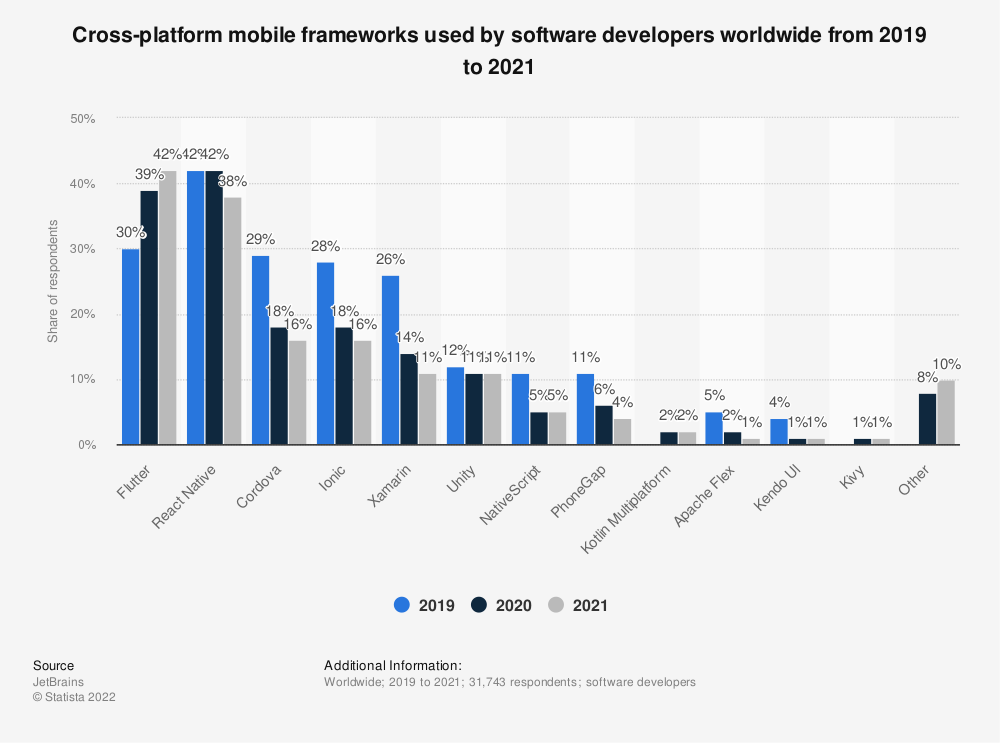
\includegraphics[height=7cm,keepaspectratio]{images/cross-platform-mobile-frameworks.png} 
  \caption{Cross-Plattform-Frameworks 2019-2021 \cite{statist_CP_Framework}}
  \label{fig:statista_cross_plattform}
\end{figure}
Abbildung \ref{fig:statista_cross_plattform} zeigt eine Statistik von JetBrains, die die Verteilung von verschiedenen Cross-Plattform-Entwicklungen zeigt. Sie zeigt eindrucksvoll wie schnell sich die Verteilung von Cross-Platform Frameworks ändern kann.
Ein Framework, das hier besonders allerdings besonders heraus sticht ist Flutter. Es ist ein Framework das erst 2017 auf den Markt gekommen ist und innerhalb von gerade einmal 4 Jahren auf einen Marktanteil von 42\% gekomm ist. Von einigen wird es schon als der neue Standard angesehen und Unternehmen wie msg. entwickeln neue Applikationen, wenn nicht offiziell anders gewünscht nur noch in Flutter.
\TODO{Fragen wie man Aussagen aus Vortrag benutzen kann}

Wegen den oben genannten Unsicherheiten und einigen anderen Gründen gibt es allerdings auch viele Entickler die immer noch nativ entwickeln. So entwickelt die Number42 alle ihre betreuten mobilen Applikationen mit den nativen Programmiersprachen. Auch die nativen Programmiersprachen entwickeln sich stetig weiter und bekommen Änderungen, die eine Entwicklung vereinfachen und beschleunigen.



Deswegen soll im folgenden verschiedene Ansätze zur Entwicklung von mobilen Anwendungen untersucht werden und dabei darauf eingegangen werdem, was die Vor- und Nachteile der verschiedenen Ansätze sind und anhand von verschiedenen Kriterien eine Einordnung liefern
\TODO{umschreiben}
Deswegen soll in dieser Arbeit drei unterschiedliche Ansätze mit beispielhaften Frameworks und Programmiersprachen betrachtet werden um am Ende vlt eine bessere Einschätzung geben zu können, wie eine solche Entscheidung ausfallen könnte und Gründe für und gegen bestimmte Ansätze geben.
\TODO{umschreiben}
Daher ist der Fokus dieser Arbeit einmal an einigen konkreten Beispielen zu untersuchen, wie der aktuelle Stand der Technologie hier ist und zu erforschen, welche Einschränkungen die Frameworks besitzen um hier auch eine gewisse Bewertung zu Benutzbarkeit als Applagentur zu untersuchen.
